\documentclass{beamer}
\usepackage{HECbeamer}
% \usepackage{pgfpages}
% \pgfpagesuselayout{4 on 1}[letterpaper, landscape, border shrink=5mm]
\title[\color{white}{MATH 60604A \S~5h - Group heteroscedasticity}]{\texorpdfstring{MATH 60604A \\Statistical modelling \\ \S~5h - Group heteroscedasticity}{MATH 60604A \\Statistical modelling \\ \S~5h - Group heteroscedasticity}}
\author{Léo Belzile}
\institute{HEC Montréal\\
Department of Decision Sciences}
\date{} 

\begin{document}
\frame{\titlepage}


\begin{frame}
\frametitle{Block covariance structure for group heteroscedasticity}
\bi 
 \item Assume that observations within groups have the same covariance structure, but the parameters of the latter differ between groups.
 \item 
 Assuming consecutive grouped measurements, the covariance matrix of all the measurements is 
 \begin{align*}
  \Co{\bs{Y}} = \begin{pmatrix}
                 \bs{\Sigma}_1 & \mathbf{O} & \cdots & \mathbf{O}\\
                  \mathbf{O} &\bs{\Sigma}_2 & \cdots & \mathbf{O} \\
                  \vdots & \ddots & \ddots & \vdots \\
                   \mathbf{O} & \mathbf{O} & \cdots & \bs{\Sigma}_m 
                \end{pmatrix}.
\end{align*}
\item We assume that $\bs{\Sigma}_1 \neq \cdots \neq \bs{\Sigma}_m$.
\ei \end{frame}
\begin{frame}{Group heteroscedasticity}
\bi
\item If the data are independent (within and between group), but heteroscedastic between groups, the matrix $\bs{\Sigma}_i = \sigma_i^2\mathbf{I}$, where $\mathbf{I}$ is the identity matrix with ones on the diagonal and zero for off-diagonal entries.  
\item In this case, there are $m$ variance parameters to estimate (one per group).
 
\item We could use a different structure for $\bs{\Sigma}_i$. \SASlang{} allows this, but the blocks cannot share parameters, so we get $m$ times the number of parameters in $\bs{\Sigma}_i$. There must be enough observations in each group to reliably estimate the covariance parameters.
\ei
\end{frame}

\begin{frame}
\frametitle{Wage discrimination in a US college}
The \code{college} data set provides the nine-month academic salary
(in thousand dollars) in 2008–2009 of professors in a college in the USA.
\bi
\item \texttt{salary}: nine month income (in thousand dollars).
\item \texttt{rank}: academic rank of the professor (assistant , associate or full).
\item \texttt{field}: categorical variable indicating whether research field is applied or theoretical.
\item \texttt{sex}: sex of individual, either man or woman.
\ei
\end{frame}
\begin{frame}
 \begin{center}
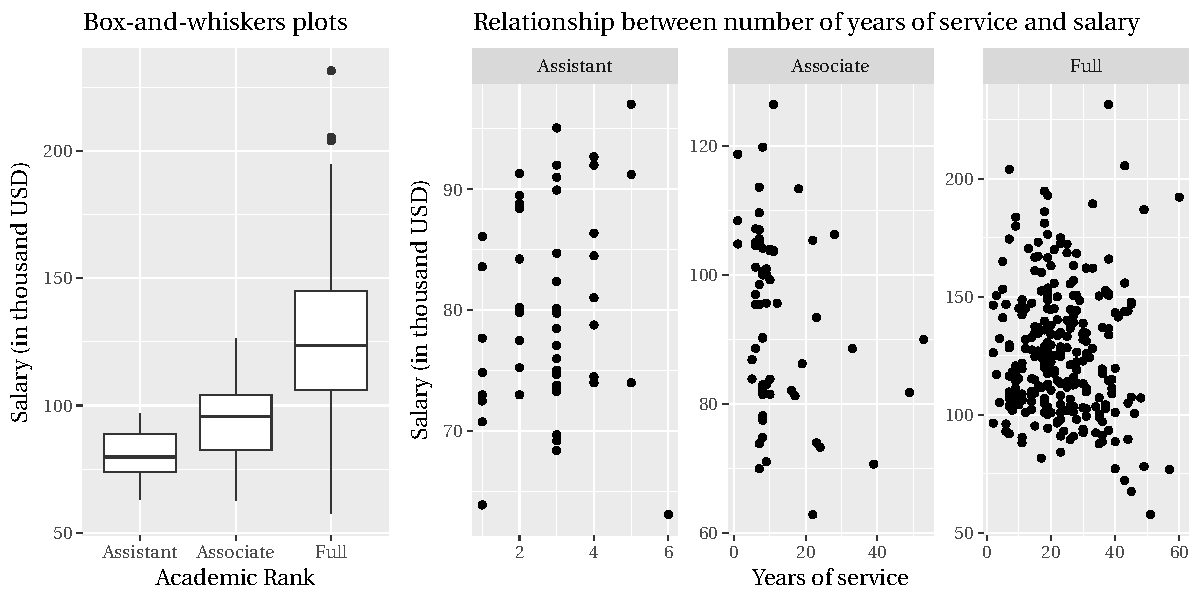
\includegraphics[width = 0.95\linewidth]{img/c5/06-correlated-salary_EDA}  
 \end{center}
The explanatory data analysis shows clear heteroscedasticity within academic rank.
\end{frame}

\begin{frame}[fragile]
\frametitle{Dealing with group heteroscedasticity}
\begin{tcolorbox}[colback=white, colframe=hecblue, title=\SASlang{} code for a different variance per group]
\begin{small}
\begin{verbatim}
proc mixed data=statmod.college plots=studentpanel;
class field rank sex;
model salary = sex field rank;
repeated / group = rank;
run;
\end{verbatim}
\end{small}
\end{tcolorbox}
The argument \texttt{repeated / group} specifies the group structure.
\end{frame}
\begin{frame}
\frametitle{Variance estimates per group and significance test}
 \begin{center}
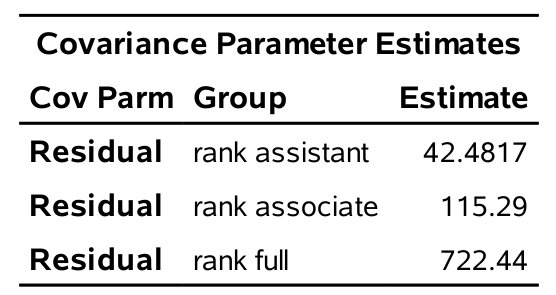
\includegraphics[width = 0.45\linewidth]{img/c5/slides6-e25}  
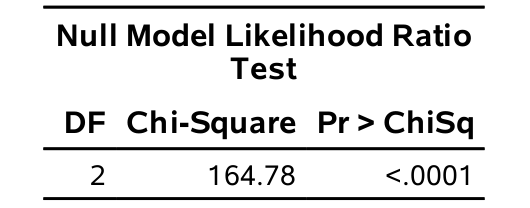
\includegraphics[width = 0.45\linewidth]{img/c5/slides6-e26}  
 \end{center}
The variance increases with rank. The likelihood ratio test shows that the model with a different group for each rank is significantly better than the linear model which assumes a constant variance for every observation.
\end{frame}
\begin{frame}{Diagnostic plots for the \texttt{profsalaries} data}
  \begin{center}
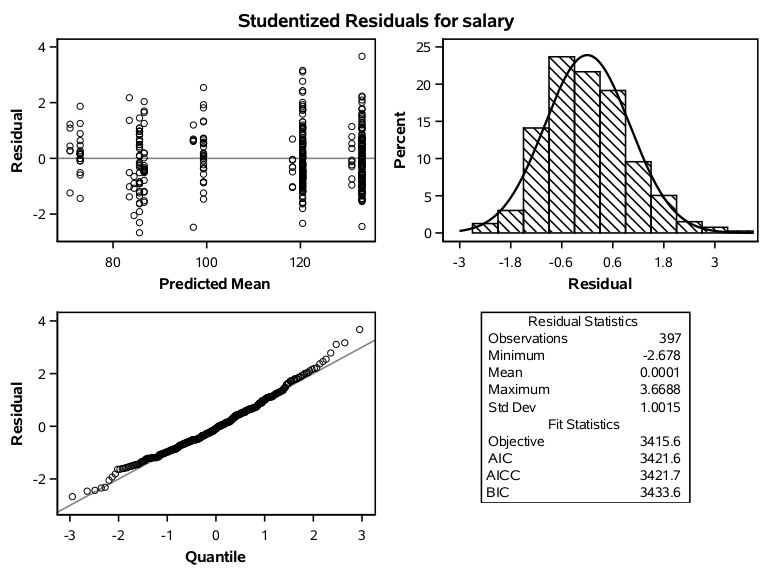
\includegraphics[width = 0.7\linewidth]{img/c5/slides6-e28}  
 \end{center}
 The residual plots show that the model captures most features well. We can be confident in our inference.
\end{frame}
\begin{frame}
 \frametitle{Mean parameter estimates}
 \begin{center}
  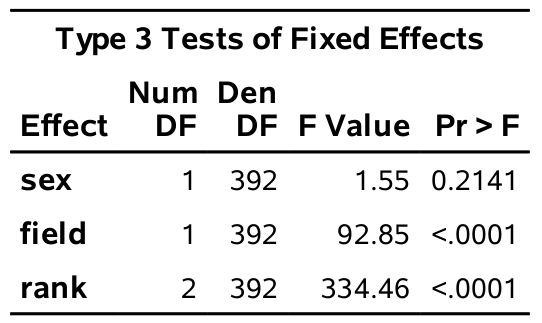
\includegraphics[width = 0.45\linewidth]{img/c5/slides6-e27}  
 \end{center}

 \bi \item 
 Solely comparing the salary of mean and women academics using a two-sample test is wrong, because rank is an important explanatory variable.
 \item  Moreover, the proportion of full professor that are women (7\%) is much lower than for assistant or associated professors (16\%)
 \item After accounting for rank and dealing with group heteroscedasticity, there is no evidence of gender gap.
 \ei
\end{frame}


% \begin{frame}[fragile]
%  \frametitle{ANOVA with different variance per group}
%  
% 
%  \ei 
% \begin{tcolorbox}[colback=white, colframe=hecblue, title=\SASlang{} code for a one-way ANOVA with  different variance per group]
% \begin{verbatim}
% proc mixed data=statmod.servqual;
% class bank;
% model reliability=bank / ddfm=satterth;
% repeated / group=bank;
% lsmeans bank / pdiff;
% run; 
% \end{verbatim}
% \end{tcolorbox}
% \end{frame}
% \begin{frame}[fragile]
% \frametitle{Two-way ANOVA with interaction, unequal variances}
% \bi \item We analyse the \code{delay} data set, with \code{time} as response variable and an interaction.
% \item We can likewise fit a different covariance parameter for each group in an ANOVA model using \code{proc mixed}.   
% \ei
% 
% \begin{tcolorbox}[colback=white, colframe=hecblue, title=\SASlang{} code for two-way ANOVA with unequal variances]
% \begin{verbatim}
% proc mixed data=statmod.delay;
% class stage delay;
% model time=stage delay stage*delay / ddfm=satterth;
% repeated / group=stage * delay;
% lsmeans stage*delay / pdiff;
% run;
% \end{verbatim}
% \end{tcolorbox}
% \end{frame}
% \begin{frame}
% \frametitle{Two-way ANOVA for \code{delay} time}
% \bi 
% %  \item The model is adjusted via REML, but we could fit multiple models with different fixed effects and compare them using maximum likelihood (through likelihood ratio tests).
% \item We included a correction to the degrees of freedom of the $F$ test (\code{ddfm=satterth}) to account for the unequal variance.
%  \item The output includes a test statistic for the equality of variance whose value is $11.76$, to be compared with a $\chi^2_5$. The $p$-value is $0.0382$, meaning that at least one variance is significatively different from the rest at the $5$\% level.
%  \item The interaction term \code{stage*delay} is not statistically significant. 
%  \item If we remove the interaction and refit the model with only main effects, both are strongly significant.
%  \ei
% \end{frame}

\end{document}
